\documentclass[dvipdfm]{beamer}
\usepackage[utf8]{inputenc}
\usepackage[brazil]{babel}
\usepackage{graphics}
\usepackage{graphicx}
\usepackage{color}
\usepackage{cite}
\usepackage{url}
\usepackage{array}
\usepackage{multirow}


\usetheme{Warsaw}
\setbeamertemplate{footline}[frame number]

\title{Como o spam afeta a comodidade do correio eletrônico}
\author{Bianca Oe\\
		Gustavo Inoue\\
		Rafael Nakanishi}
\institute{Instituto de Ciências Matemáticas e Computação}

\AtBeginSection[]
{
 \begin{frame}<beamer>
	\begin{scriptsize}
 	\tableofcontents[currentsection,hideothersubsections]
	\end{scriptsize}
 \end{frame}
}

\newcolumntype{C}[1]{>{\centering\let\newline\\\arraybackslash\hspace{0pt}}m{#1}}
\setbeamerfont{footnote}{size=\fontsize{5pt}{6pt}}

\begin{document}

\begin{frame}
	\titlepage
\end{frame}

\begin{frame}
	\begin{scriptsize}
		\tableofcontents[hidecurrentsubsection,hideothersubsections]
	\end{scriptsize}
\end{frame}

\section{O que é Spam}
\begin{frame}{O que é Spam}
	\begin{itemize}
		\item Sp(iced H)am, 1937
		\item Monty Python, 1970 \footnote{\url{http://www.youtube.com/watch?v=anwy2MPT5RE}}
		\item “spam spam spam spam spam spam spam baked beans  spam spam spam and  spam”
	\end{itemize}

	\begin{figure}[h]
		\centering
		
\includegraphics[width=3cm]{Imagens/spam/spam.png}
	\end{figure}
\end{frame}

\begin{frame}{O que é spam}
	\begin{itemize}
		\item E-mail indesejado ou inapropriado
			\begin{table}
			\begin{flushleft}
				\begin{tabular}{p{0.25\textwidth} p{0.25\textwidth} p{0.25\textwidth}}
					Fraude & Adulto & Financeiro \\
					Farmacêuticas & Phishing & Diplomas \\
					Software & Malware & Jogos \\
					Outros & Ações & Réplicas \\
					Relacionamento\\
				\end{tabular}
			\end{flushleft}
			\end{table}

		\item Enviado independentemente da localização do púbico-alvo
	\end{itemize}
\end{frame}

\section{Filtros de Spam}
\begin{frame}{Filtros de Spam}
	\begin{itemize}
		\item Separar mensagens de propagandas
		\begin{itemize}
			\item Spam $\times$ Ham
		\end{itemize}
	\end{itemize}
	\begin{figure}[h]
		\centering
		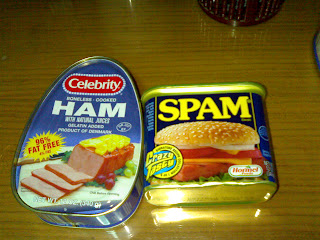
\includegraphics[width=5cm]{Imagens/spam/spamvsham.jpg}
	\end{figure}
\end{frame}

\subsection{Baseado na estrutura do texto} 
\begin{frame}{Baseado na estrutura do texto}
	\begin{itemize}
		\item Cadeias específicas no cabeçalho do texto
		\begin{itemize}
			\item Tipo de conteúdo
			\item	Língua em que a mensagem foi escrita
		\end{itemize}
		\item Dados de baixo nível
		\item Critérios subjetivos
		\begin{itemize}
			\item Quantidade de imagens por texto
		\end{itemize}
	\end{itemize}
\end{frame}

\subsection{Whitelist/Verificação} 
\begin{frame}{\emph{Whitelist}/Verificação}
	\begin{itemize}
		\item Lista de endereços válidos
		\item ``Challenge''
		\item Problema para usuário legítimo
		\item \emph{Corlive}
	\end{itemize}
	\begin{figure}
		\centering
		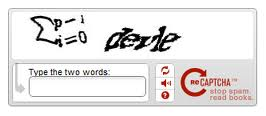
\includegraphics[height=1.5cm]{Imagens/random/recaptcha.jpg}
	\end{figure}
\end{frame}

\subsection{Distribuição adaptativa de blacklist}
\begin{frame}{Distribuição adaptativa de \emph{blacklist}}
	\begin{itemize}
		\item Mensagens classificadas como spam por usuários ou pelo próprio servidor
		\item Baseado em técnicas estatísticas
		\begin{itemize}
			\item Mutações no e-mail não devem impedir classificação como spam
		\end{itemize}
		\item Performance baixa
		\item Pyzor
	\end{itemize}
\end{frame}

\subsection{Ranking baseado em regras}
\begin{frame}{Ranking baseado em regras}
	\begin{itemize}
		\item Classificação baseada em ranking
		\item Correspondência de regras
		\item Regras constantes
		\begin{itemize}
			\item Endereço falso
		\end{itemize}
		\item Regras variáveis
		\begin{itemize}
			\item Propaganda
		\end{itemize}
		\item SpamAssassin
	\end{itemize}
	\begin{figure}
		\centering
		
\includegraphics[height=2cm]{Imagens/random/spamassassin.png}
	\end{figure}
\end{frame}

\subsection{Filtro Bayesiano}
\begin{frame}{Filtro Bayesiano}
	\begin{itemize}
		\item Baseado em modelos Bayesianos de probabilidade
		\item Dicionário de palavras
		\begin{itemize}
			\item Probabilidade da palavra pertencer a um spam
			\item Cálculo da probabilidade da mensagem ser spam
		\end{itemize}
		\item Simples
		\item Automatizável
		\begin{itemize}
			\item Capacidade de aprendizado
		\end{itemize}
		\item SpamBayes
		\item Gmail, MSN Hotmail, Yahoo! mail
	\end{itemize}
\end{frame}

\subsection{Filtro Markoviano}
\begin{frame}{Filtro Markoviano}
	\begin{itemize}
		\item Cadeias de Markov
		\item Baseado em frases
		\item Maior desempenho
		\item CRM114
	\end{itemize}
\end{frame}

\subsection{Gmail}
\begin{frame}{Gmail}
	\begin{itemize}
		\item \emph{Community clicks}
		\item Autenticação de endereço
		\item Filtros personalizados
		\item Google Book Search
	\end{itemize}
	\begin{figure}
		\centering
		
\includegraphics[height=3cm]{Imagens/spam/spamimagem.jpg}
	\end{figure}	
\end{frame}

\begin{frame}{Gmail}
	\begin{figure}
		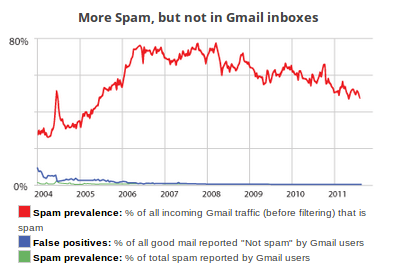
\includegraphics[height=5cm]{Imagens/gmail/spamchart.png} \footnote{Retirado de \url{http://www.google.com/mail/help/fightspam/spamexplained.html}}
	\end{figure}
\end{frame}

\section{Casos reais}

\subsection{Coxinha em promoção}
\begin{frame}{Coxinha em promoção}
	\begin{itemize}
		\item Jornalista Lúcia Guimarães
		\begin{itemize}
			\item Mora em Nova Iorque
		\end{itemize}
		\item Recebe e-mail de uma promoção de um salgado
		\begin{itemize}
			\item Cidade Baixa de Porto Alegre
			\item 50\% de desconto
			\begin{itemize}
				\item De R\$12.50 por R\$6.00
			\end{itemize}
		\end{itemize}
		\item R\$4.000 a passagem para Porto Alegre
	\end{itemize}
\end{frame}

\begin{frame}{Coxinha em promoção}
``Se alguma corporação estiver espionando minha correspondência eletrônica com base num algoritmo, pode montar um perfil em que: 
		Eu como coxinha em Porto Alegre; 
		corto o cabelo em Belo Horizonte; 
		compro câmeras no Estado do Maine; 
		passo os fins de semana em Búzios; 
		encomendo pornografia do Estado de Nevada. 
		Enfim, sou uma verdadeira cidadã do mundo, cheia de caprichos e perversões.''
\end{frame}

\subsection{Amizades via spam}
\begin{frame}{Amizades via spam}
	\begin{itemize}
		\item Início em 29 de fevereiro
		\item Um grupo de milhares de pessoas recebeu um spam
		\begin{itemize}
			\item Utilização de listserv
			\item Ao clicar em "Responder para todos", a mensagem era encaminhada para todo o grupo
		\end{itemize}
		\item Várias pessoas mandaram mensagens pedindo, mandando e obrigando a tirá-los da lista de e-mails
		\begin{itemize}
			\item Sr. Clark chegou a mandar 12 mensagens em uma hora
			\item Acabou recebendo ligações de queixas de várias pessoas
		\end{itemize}
		\item Starwood Hotel era um dos integrantes da lista
		\begin{itemize}
			\item O hotel achou que as pessoas não queriam mais receber informativos do hotel
			\item Alguém acabou achando que a culpa era do hotel
			\item Chegou a ocorrer ameça envolvendo a polícia italiana
		\end{itemize}
	\end{itemize}
\end{frame}

\begin{frame}{Amizades via spam}
	\begin{itemize}
		\item As pessoas perceberam que continuar respondendo só levaria a manter o ciclo de spam
		\item Um escritor de Londres sugeriu que eles saíssem para se encontrarem
		\item Várias pessoas aderiram
		\item Grupo no \emph{LinkedIn}
		\begin{itemize}
			\item \emph{Unified by spam - the Social Experiment}
			\url{http://www.linkedin.com/groups/Unified-Spam-Social-Experiment-4336202?gid=4336202\&mostPopular=\&trk=tyah}
		\end{itemize}
	\end{itemize}
\end{frame}

\section{Estudo de caso}
\subsection{Apresentação do caso}
%\begin{frame}{Estudo de caso}
%\begin{itemize}
%	\item Baseado em fatos
%	\item Juliano
%	\begin{itemize}
%		\item Professor de uma Universidade renomada
%		\item Ministra determinada disciplina num determinado semestre
%	\end{itemize}
%	\item Eduardo
%	\begin{itemize}
%		\item Pós-graduando sobre tutoria de Juliano
%		\item Iminência de defender o mestrado
%		\item Auxilia Juliano com a disciplina
%	\end{itemize}
%\end{itemize}
%\end{frame}

%\begin{frame}{Estudo de caso}
%\begin{itemize}
%	\item Média final da disciplina composta por projetos e nenhuma prova
%	\begin{itemize}
%		\item Projetos lançados ao longo do semestre
%	\end{itemize}
%	\item Testes são necessários pra comprovar eficiência e são realizados em máquinas específicas
%	\item Máquina compartilhadas
%	\begin{itemize}
%		\item Flutuação do resultado
%	\end{itemize}
%\end{itemize}
%\end{frame}

%\begin{frame}{Estudo de caso}
%	\begin{itemize}
%		\item Alocação dos recursos feito pelo professor
%		\begin{itemize}
%			\item Horários não levavam em conta disponibilidade dos alunos
%			\item Grupos não conseguiram terminar os testes
%			\item Vários e-mails pedindo nova alocação
%		\end{itemize}
%		\item Juliano pede a Eduardo para mandar e-mails para os alunos avisando sobre as mudanças
%		\item Eduardo faz o que foi pedido, mas percebe que ainda haverá várias mudanças
%	\end{itemize}
%\end{frame}

%\begin{frame}{Estudo de caso}
%\begin{itemize}
%	\item O \emph{site} da disciplina poderia ser usado para avisar sobre as mudanças
%	\begin{itemize}
%		\item Apenas Juliano possuía acesso para realizar alterações
%	\end{itemize}
%	\item Os e-mails de modificações poderia ser mandado apenas para os grupos afetados
%	\item Eduardo avisa Juliano que mandar a todos se trataria de um spam
%	\begin{itemize}
%		\item Juliano diz ser irrelevante
%	\end{itemize}
%\end{itemize}
%\end{frame}

\begin{frame}{Contexto}
	\hspace{1pc}Eduardo, é orientando de Juliano, professor de uma universidade, e está na iminência de defender sua tese de mestrado.
	Em determinado semestre, Juliano ficou responsável por ministrar uma disciplina, da qual Eduardo era monitor, que possuia vários projetos.
	
	\hspace{1pc}Nos projetos, para comprovar a eficiência da solução, os alunos deveriam fazer vários testes em máquinas específicas fornecidas pela instituição.
	
	\hspace{1pc}O professor decidiu alocar períodos de tempo para cada grupo, para que não houvesse flutuações nos resultados.
	Se outros grupos utilizassem os recursos em um período que não fosse seu, seriam penalizados.
\end{frame}

\begin{frame}{Contexto}
	\hspace{1pc}Foi feita uma alocação inicial, escolhida por Juliano, porém os horários não levavam em conta a disponibilidade dos alunos, o que causou vários transtornos, fazendo os alunos pedirem pela remarcação dos mesmos.
	
	\hspace{1pc}Juliano decidiu atender ao pedido dos alunos e disse para Eduardo mandar um e-mail aos alunos para lhes avisar sobre todas as mudanças feitas.
	
	\hspace{1pc}Após alguns envios, Eduardo percebeu que ainda aconteceriam várias modificações e que isso geraria uma grande quantidade de mensagens que não eram importantes para todos os alunos, como, por exemplo, os alunos que já haviam realizado os testes de forma bem sucedida.
\end{frame}

\begin{frame}{Contexto}
	\hspace{1pc}Era possível utilizar o site da disciplina para informar as modificações, assim como foi feito para a primeira alocação. 
	Mas somente o professor poderia fazê-lo, e, quando Eduardo sugeriu esta possibilidade, Juliano não pareceu disposto a gastar seu tempo de pesquisa para atualizar o documento que continha os horários reservados.
	
	\hspace{1pc}O orientando não queria irritar seu orientador às vésperas de sua defesa, já que isso poderia prejudicá-lo. 
	Por outro lado, se estivesse no lugar dos alunos, se sentiria incomodado pelo spam acadêmico recebido.
\end{frame}

\begin{frame}{Dados relevantes}
	\begin{itemize}
			\item Juliano
				\begin{itemize}
					\item Professor
					\item Orientador de Eduardo
					\item Pesquisador da universidade
				\end{itemize}
			\item Eduardo
				\begin{itemize} 
					\item Mestrando prestes a defender sua tese
					\item Monitor da disciplina
					\item Orientando de Juliano
				\end{itemize} 
			\item Alunos
				\begin{itemize} 
					\item	Matriculados na disciplina ministrada por Juliano e monitorada por Eduardo
					\item Insatisfeitos com a quantidade de e-mails recebidos
				\end{itemize}
		\end{itemize}
\end{frame}

\begin{frame}{Possíveis decisões}
	\begin{itemize}
		\item Insistir para Juliano modificar o documento no site
		\item Enviar o e-mail das modificações apenas para os interessados
		\item Enviar o e-mail das modificações para todos os alunos
		\item	Guardar as modificações e enviá-las em blocos para todos os alunos
	\end{itemize}
\end{frame}

\subsection{Códigos da ACM violados}
\begin{frame}{Códigos da ACM violados}
		\begin{itemize}
			\item ``Contribuir para o bem-estar humano e da Sociedade''\\
				
			\item ``Procurar alcançar a maior qualidade, eficácia de dignidade tanto nos processos como nos produtos do trabalho profissional''\\
				
			%\item ``Adquirir e manter competência profissional''\\
				
		\end{itemize}
\end{frame}

\subsection{Obrigações, benefícios e vulnerabilidades}
\begin{frame}{Tabela de Obrigações}
	\begin{table}[h!]
		\centering
		\begin{tabular}{@{\extracolsep{\fill}} l C{0.2\textwidth} C{0.2\textwidth} C{0.2\textwidth}}
			\hline
								&	\textbf{Juliano}		&	\textbf{Eduardo}	&	\textbf{Alunos}\\	
			\hline
			\textbf{Juliano}	&	Pesquisar	&	Orientar para a docência	&	Passar conhecimento\\
			\hline
			\textbf{Eduardo}	&	Obedecer \linebreak \linebreak Auxiliar na disciplina	&	Prezar pela pós-graduação	&	Avisar sobre mudanças\\
			\hline
			\textbf{Alunos}	&	Ser aprovado na disciplina	&			&	Manter boas notas\\
			\hline
		\end{tabular}
	\end{table}
\end{frame}

\begin{frame}{Grafo de obrigações}
	\begin{figure}
		\centering
		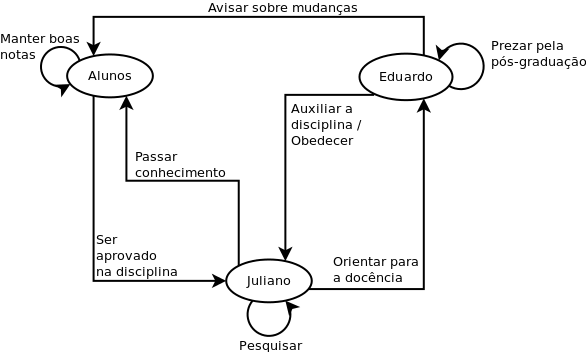
\includegraphics[height=4cm]{diagramas/grafo-de-obrigacoes.png}
	\end{figure}
\end{frame}

\begin{frame}{Tabela de benefícios}
	\begin{tiny}
	\centering
		\begin{table}[h!]
			\centering
			\begin{tabular}{@{\extracolsep{\fill}}C{0.17\textwidth}  C{0.17\textwidth} C{0.17\textwidth} C{0.17\textwidth} C{0.17\textwidth} C{0.17\textwidth}}
				\hline
				 & \textbf{Insistir para Juliano modificar no site} & \textbf{Enviar apenas para os interessados} & \textbf{Enviar para todos} & \textbf{Enviar blocos de modificações}\\
				\hline
				Alunos interessados & Não receberão nenhum e-mail \linebreak \linebreak Serão notificados & Serão notificados & Serão notificados & Receberão menos e-mails \linebreak \linebreak Serão notificados\\
				\hline
				Alunos não interessados & Não receberão nenhum spam & Não receberão nenhum spam &  & Receberão menos e-mails\\
				\hline
				Eduardo & Não precisa enviar os e-mails & & & Envia menos e-mails \\
				\hline
				Juliano & & Não envia e-mails & Não envia e-mails & Não envia e-mails \\
				\hline
			\end{tabular}
		\end{table}
	\end{tiny}
\end{frame}

\begin{frame}{Tabela de vulnerabilidades}
	\begin{tiny}
		\begin{table}[h!]
			\centering
			\begin{tabular}{@{\extracolsep{\fill}}C{0.15\textwidth} C{0.15\textwidth} C{0.15\textwidth} C{0.15\textwidth} C{0.15\textwidth}}
				\hline
				& \textbf{Insistir para Juliano modificar o documento no site} & \textbf{Enviar apenas para os interessados} & \textbf{Enviar para todos} & \textbf{Enviar blocos de modificações}\\
				\hline
				Alunos interessados & & & Recebe spam & Recebe spam \\
				\hline
				Alunos não interessados & & & Recebe spam & Recebe spam \\
				\hline
				Eduardo & & Envia e-mails & Envia e-mails & Envia e-mails \\
				\hline
				Juliano & Precisa modificar o documento & & &\\
				\hline
			\end{tabular}
		\end{table}
	\end{tiny}
\end{frame}

\begin{frame}{Tabela de obrigações afetadas}
	\begin{tiny}
		\begin{table}
			\begin{tabular*}{\textwidth}{@{\extracolsep{\fill}} C{0.09\textwidth} C{0.08\textwidth} C{0.08\textwidth} C{0.115\textwidth} C{0.115\textwidth} C{0.115\textwidth} C{0.115\textwidth}}
				\cline{2-7}
				& & & \textbf{Insistir para Juliano modificar no site} & \textbf{Enviar apenas para os interessados} & \textbf{Enviar para todos} & \textbf{Enviar blocos de modificações}\\
				\hline
				\multirow{3}{*}{Eduardo}  & Para ele mesmo & Prezar pela pós-graduação & - - & - - & - & - \\
				\cline{2-7}
						& Juliano & Obedecer & - & + & + + & + \\
				\cline{2-7}
						& Alunos & Notificar & + - & + & + & + \\
				\hline
				Juliano & Para ele mesmo & Pesquisar & - - &  &  & \\
				\hline
			\end{tabular*}
		\end{table}	
	\end{tiny}
\end{frame}

\subsection{Decisão consensual}
\begin{frame}{Decisão consensual}
	\begin{itemize}
		\item Eduardo tentar convencer Juliano a atualizar o site.
		\begin{itemize}
			\item Se a relação com o orientador ficar ruim, mandar as notificações em blocos
		\end{itemize}
	\end{itemize}
\end{frame}


\section{Links interessantes}
\begin{frame}{Links interessantes}

	\begin{itemize}
		\item Yahoo Visualization Tool
		\begin{itemize}
			\item \url{http://visualize.yahoo.com/mail/}
		\end{itemize}
		\item Google Postini Services
		\begin{itemize}
			\item \url{http://www.google.com/postini/threat_network.html}
		\end{itemize}
	\end{itemize}
\end{frame}

\section{Referências}
\begin{frame}{Referências}
	\begin{itemize}
		\item [1] Monty Python, \emph{Spam}, 1970, \url{http://www.youtube.com/watch?v=anwy2MPT5RE} 
	\end{itemize}
\end{frame}

\end{document}
